\documentclass{article}

%%%%%%%% CREATE DOCUMENT STRUCTURE %%%%%%%%
%% Language and font encodings
\usepackage[english]{babel}
\usepackage[utf8]{inputenc}
\usepackage[T1]{fontenc}
%\usepackage{subfig}

%% Sets page size and margins
\usepackage[a4paper,top=3cm,bottom=2.5cm,left=2.5cm,right=2.5cm,marginparwidth=1.75cm]{geometry}

%% Useful packages
\usepackage{comment}
\usepackage{indentfirst}
\usepackage{lipsum}
\usepackage{amsmath}
\usepackage{amssymb}
\usepackage{mathrsfs}
\usepackage{amsfonts}
\usepackage{graphicx}
\usepackage[colorinlistoftodos]{todonotes}
\usepackage[colorlinks=true, allcolors=blue]{hyperref}
\usepackage{caption}
\usepackage{subcaption}
\usepackage{sectsty}
%\usepackage{apacite}
\usepackage{cite}
\usepackage{float}
\usepackage{titling} 
\usepackage{blindtext}
%\usepackage[square,sort]{natbib}
%\usepackage[sort]{natbib}
\usepackage{epstopdf}
\usepackage[colorinlistoftodos]{todonotes}
\usepackage{xcolor}
\definecolor{darkgreen}{rgb}{0.0, 0.4, 0.0}
\setlength{\marginparwidth}{2cm}
\usepackage{pdflscape}
\usepackage{tabularx}

\usepackage{helvet}
\renewcommand{\familydefault}{\sfdefault}
\linespread{1.25}
\setlength{\parindent}{1.35cm}


%%%%%%%%%%%%%%%%%%%%%%%%%%%%%%%%%%%%%%%%%%


\begin{document}

\begin{titlepage}
\newcommand{\HRule}{\rule{\linewidth}{0.5mm}}                           % horizontal line and its thickness
\center

% Title of the report


\includegraphics[width=0.8\textwidth]{concordia_logo.png}\\[0.2cm]  % Concordia Logo

\HRule \\[0.8cm]
\textbf{\Large SOEN 6841: SOFTWARE PROJECT MANAGEMENT}\\[0.2cm]
\HRule \\
\vfill

%Title of the Research
\textbf{\Large How can I motivate contributors to
participate in project retrospective
analysis? }\\
%\textbf{\Large ELEMENT AND TIME DELAY }\\[0.9cm]
\vfill
\textbf{\large Task Analysis and Synthesis \\  Student ID: 40226298 }\\
\vfill


\text{\large Nov 1, 2023}\\
\vfill
\end{titlepage}
\newpage
\tableofcontents
\newpage

\section{ABSTRACT}
    Effective project retrospective analysis is crucial for continuous improvement in project management. This report explores strategies to motivate contributors to actively participate in post-project assessments, addressing the challenge of reluctance and the common aversion to additional meetings. By highlighting personal, project-oriented, and organizational benefits, project leaders can encourage enthusiastic engagement. The report emphasizes the importance of focusing on both positive aspects and areas for improvement, fostering a constructive atmosphere. Additionally, it discusses the role of retrospective analyses in building better projects, driving process improvements, and enhancing overall efficiency. Commitment to implementing key recommendations ensures active participation and contributes to better project outcomes. At the organizational level, the report highlights the broader benefits, including increased efficiency, organizational learning, and opportunities for professional growth. By recognizing and addressing the concerns of contributors, project leaders can create a conducive environment for successful retrospective analyses.


    Motivating contributors to participate in project retrospective analysis is crucial for continuous improvement and organizational growth. This report explores strategies to engage reluctant contributors by highlighting personal, project-oriented, and organizational benefits. It emphasizes the importance of addressing tension, crisis, and drama from past projects to foster a positive mindset for future endeavors. Additionally, it discusses the significance of capturing lessons learned to build better projects and outlines the benefits of disciplined post-project analysis for the organization.

\begin{comment}
\begin{figure}[H]
\includegraphics[width=\textwidth]{image path}
\label{fig:igotvm}
\caption*{Table 1 : caption}
\end{figure}
\end{comment}

\newpage

\section{INTRODUCTION}
Project retrospective analysis plays a pivotal role in evaluating the success and areas for improvement at the conclusion of a project or iteration. It provides a structured opportunity for project teams to reflect on their recent experiences, identify opportunities for improvement, and make informed decisions for future endeavors. By reviewing the project facts, setting the stage, gathering data, generating insights, deciding on the next steps, and closing the retrospective, teams can effectively assess what worked well and what could have been better. This report aims to explore the strategies for motivating contributors to participate in project retrospective analysis by emphasizing the personal, project-oriented, and organizational benefits. It will delve into the significance of addressing tension, crisis, and drama from past projects to foster a positive mindset for future endeavors, capturing lessons learned to build better projects, and outlining the benefits of disciplined post-project analysis for the organization. Through this exploration, project leaders can gain insights into engaging reluctant contributors and ultimately contribute to the growth and success of future projects and the organization as a whole.

\subsection{Motivation}
The investigation into motivating contributors to participate in project retrospective analysis is driven by the recognition of the critical role that team motivation plays in the success of a project. While the project retrospective meeting provides an opportunity to analyze both successes and failures, the active participation of team members is essential for the team and organization to improve their work going forward Motivation is predominantly about emotion, and it is crucial to create a blameless environment where team members feel comfortable expressing their feelings and actions without fear of punishment. By understanding the current environment and prioritizing actions, project leaders can optimize team motivation by addressing factors such as autonomy and mastery, which significantly impact the motivation of team members. The investigation into this problem is also motivated by the need to introduce concepts and exercises that can effectively engage team members in the retrospective process, fostering a sense of closure for completed projects and turning past mistakes into learning opportunities. Overall, the motivation behind this investigation stems from the desire to enhance team motivation, create a positive working environment, and drive continuous improvement within the organization.

\subsection{Problem Statement}
Despite the inherent value of project retrospective analysis in driving continuous improvement, a significant challenge persists — the reluctance of contributors to actively participate in this essential process. The tendency to view retrospectives as additional meetings, coupled with the eagerness to transition swiftly to the next project, hampers the effectiveness of post-project assessments. The critical question arises: How can project leaders motivate contributors to engage wholeheartedly in retrospective analysis, ensuring a comprehensive exploration of lessons learned and the identification of areas for improvement? This problem statement aims to address the precise challenge of fostering enthusiasm and commitment among team members for meaningful participation in project retrospective analyses.

    \newpage

\subsection{Objectives}
\paragraph*{Motivate Contributors:}
The primary objective of this investigation is to develop effective strategies that motivate contributors to actively participate in project retrospective analyses. By addressing the question of "What’s in it for me?" at the individual level, we aim to foster a sense of purpose and engagement among team members during these crucial assessments.

\paragraph*{Enhance Learning and Improvement:} Our goal is to facilitate a culture of continuous improvement within project management by ensuring that retrospective analyses are thorough and insightful. This involves encouraging open discussions about both successes and challenges, leading to the identification of valuable lessons learned.

\paragraph*{Improve Project Outcomes:} By actively involving contributors in the retrospective process and committing to implementing key recommendations, the investigation seeks to improve the outcomes of future projects. Shorter project durations, increased efficiency, and reduced confusion are anticipated benefits.
    
\paragraph*{Benefit Individuals and Organizations:} The investigation aims to benefit both individual contributors and the organizations they work for. At the individual level, active participation in retrospective analyses provides contributors with opportunities for personal and professional growth. At the organizational level, the outcomes contribute to increased efficiency, stability, and a positive work environment.

\paragraph*{Promote a Culture of Recognition:} Through successful retrospective analyses, the investigation aspires to create visibility for contributors, identifying new project leaders and subject matter experts. This recognition not only benefits individuals but also contributes to the overall success of future projects.

\paragraph*{Drive Organizational Learning:} The investigation seeks to contribute to the accumulation of intellectual capital within the organization. By capturing and applying lessons learned from retrospective analyses, we aim to foster a stable and pleasant work environment that aligns with the organization's long-term goals.
\\
\\The ultimate aim of these objectives is to establish a framework that transforms project retrospective analyses into not just obligatory exercises but into catalysts for sustained improvement, benefiting both contributors and the organizations they serve.


\begin{figure}[H]
\caption{Project retrospective meeting}
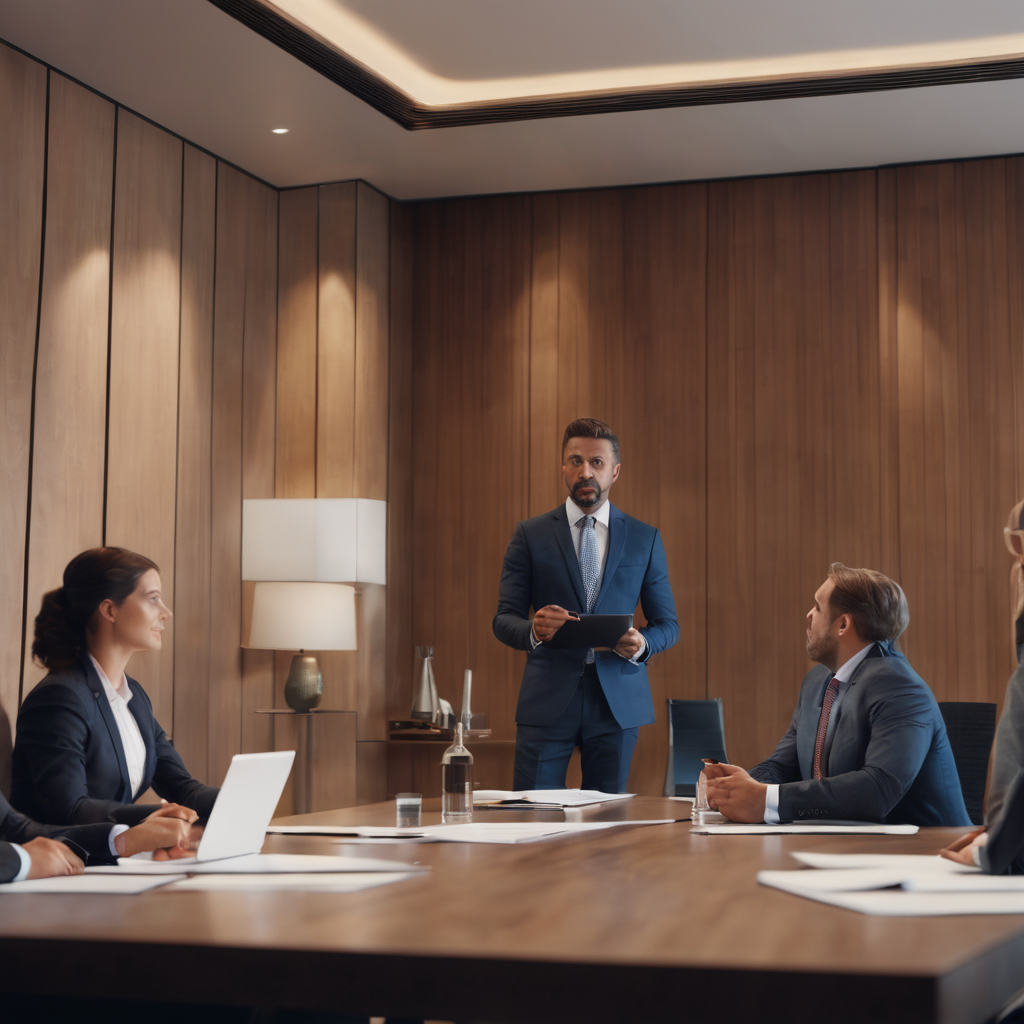
\includegraphics[width=\textwidth]{Project retrospective.png}
\label{fig: project meeting}
\end{figure}


\begin{comment}
\begin{enumerate}
    \item \textbf{TVM} is directly associated with the \textbf{Ticket} and \textbf{iGoCard}.
    \item \textbf{Ticket} is directly associated with \textbf{PaymentMode} as it is the next step after choosing the desired ticket by the customer.
    \item Same is for \textbf{iGoCard}.
    \item \textbf{PaymentMode} then is associated with the \textbf{Payment} as it is needed before redirecting to the \textbf{PaymentGateway}.
    \item \textbf{Payment} is directly associated with \textbf{Receipt} and \textbf{Gateway} class as Payment is the class that gets the final acknowledgment from the Gateway.
\end{enumerate}

\begin{enumerate}
    \item To set the language, the user selects their preferred language on the TVM, which sends a message to the iGo TVM object.
    \item Choosing an option type involves the user selecting if they want to purchase a ticket or recharge card. This sends a message to the iGo TVM object to select the option type.
    \item If chosen recharge card, it asks the user to select the age group they belong to and prices would be different for each age group.
    \end{enumerate}
\end{comment}


\newpage

\section{BACKGROUND MATERIAL}
\begin{comment}
    
In order to develop an interactive and user-friendly application, the Graphical User Interface and Backend for the iGo TVM application is implemented in the Python programming language utilising Tkinter and customTkinter python modules. The two main use cases are purchasing a ticket and recharging to a TVM card. Other components, such as payment, language selection options, and the ability to choose from a variety of age groups and fare types, have been included to assure the proper operation of these use cases.

\end{comment}
\subsection{Subject 1}

\begin{comment}

\begin{figure}[H]
\includegraphics[width=\textwidth]{t1_1.png}
\label{fig:t1}
\caption{Home Sceen of iGo TVM}
\end{figure}

\begin{figure}[H]
\includegraphics[width=\textwidth]{t1_2.png}
\label{fig:t1}
\caption{Welcome Sceen of iGo TVM}
\end{figure}

\end{comment}

\subsection{Subject 2}
\begin{comment}
    
\begin{figure}[H]
    \begin{center}
        \includegraphics[width=.3\textwidth]{t6_2.png}
        \includegraphics[width=.3\textwidth]{t8_2.png}
        \includegraphics[width=.3\textwidth]{t9_2.png}
    \end{center}
    \caption{Message Boxes for error messages}
\end{figure}
\end{comment}

\newpage
\section{METHODS \& METHODOLGY}

\subsection{How did we approach the problem?}

\subsection{What techniques are used in analysis of results}

\begin{comment}
    
\begin{center}
\begin{tabular}{ |c|c|c|c| } 
     \hline
     Sr No.\# & Test Cases & Result \\
     \hline
     1  & Test that a user can select their preferred language  &   \\
     \hline
     2  & Test that a user can recharge their TVM card using cash  &   \\
     \hline
     3  & Test that a user can recharge their TVM card using credit/debit card  &   \\
     \hline
     4  & Test that a user can purchase a ticket using cash  &   \\
     \hline
     5  & Test that a user can purchase a ticket using credit/debit card  &   \\
     \hline
     6  & Test that a user inserts amount equal or more than the payment amount &   \\
     \hline
     7  & Test that a user can select their preferred receipt option  &   \\
     \hline
     8  & Test that a user can enters a valid e-mail id &    \\
     \hline
     9 &  Test that a user inputs only numbers when inserting amount &    \\
     \hline
\end{tabular}
\captionof*{table}{Table 8 : Test Cases to verify}
\end{center}
    
\subsection{Sample Data Test cases}

\subsubsection{Test Case \#1}
\noindent\textbf{Test Case} : Test that a user can select their preferred language.\\
\textbf{Steps}:
\begin{enumerate}
    \item Select any of the language options given on main screen.
    \item Press the next button.
    \item Verify that the TVM displays information in the chosen language.
\end{enumerate}
\textbf{Result} : Test Case Passed

\begin{figure}[H]
    \begin{center}
        \includegraphics[width=.4\textwidth]{t1_1.png}
        \includegraphics[width=.4\textwidth]{t1_2.png}
        \includegraphics[width=.4\textwidth]{t1_3.png}
        \includegraphics[width=.4\textwidth]{t1_4.png}
    \end{center}
    \caption{Test case 1 images}
\end{figure}


\subsubsection{Test Case \#2}
\noindent\textbf{Test Case} : Test that a user can recharge their TVM card using cash.\\
\textbf{Steps}:
\begin{enumerate}
    \item Press Recharge Card button and press next.
    \item Select Any age group and press next.
    \item Select fare type you want to recharge and press next.
    \item Select pay by cash and press next.
    \item Input amount to be paid and make sure it is more or equal to the billing amount.
    \item Verify that the cash payment successful message for recharging card printed on screen.
\end{enumerate}
\textbf{Result} : Test Case Passed

\begin{figure}[H]
    \begin{center}
        \includegraphics[width=.3\textwidth]{t2_1.png}
        \includegraphics[width=.3\textwidth]{t2_2.png}
        \includegraphics[width=.3\textwidth]{t2_3.png}
        \includegraphics[width=.3\textwidth]{t2_4.png}
        \includegraphics[width=.3\textwidth]{t2_5.png}
        \includegraphics[width=.3\textwidth]{t2_6.png}
    \end{center}
    \caption{Test case 2 images}
\end{figure}


\subsubsection{Test Case \#3}
\noindent\textbf{Test Case} : Test that a user can recharge their TVM card using credit/debit card.\\
\textbf{Steps}:
\begin{enumerate}
    \item Press Recharge Card button and press next.
    \item Select Any age group and press next.
    \item Select fare type you want to recharge and press next.
    \item Select pay by card and press next.
    \item Verify that the card payment successful message for recharging card printed on screen.
\end{enumerate}
\textbf{Result} : Test Case Passed

\begin{figure}[H]
    \begin{center}
        \includegraphics[width=.3\textwidth]{t2_1.png}
        \includegraphics[width=.3\textwidth]{t2_2.png}
        \includegraphics[width=.3\textwidth]{t2_3.png}
        \includegraphics[width=.3\textwidth]{t3_1.png}
        \includegraphics[width=.3\textwidth]{t3_2.png}
    \end{center}
    \caption{Test case 3 images}
\end{figure}


\subsubsection{Test Case \#4}
\noindent\textbf{Test Case} : Test that a user can purchase a ticket using cash.\\
\textbf{Steps}:
\begin{enumerate}
    \item Press Purchase a ticket button and press next.
    \item Select fare type you want to recharge and press next.
    \item Select pay by card and press next.
   \item Input amount to be paid and make sure it is more or equal to the billing amount.
    \item Verify that the cash payment successful message for purchasing a ticket printed on screen.
\end{enumerate}
\textbf{Result} : Test Case Passed

\begin{figure}[H]
    \begin{center}
        \includegraphics[width=.3\textwidth]{t4_1.png}
        \includegraphics[width=.3\textwidth]{t4_2.png}
        \includegraphics[width=.3\textwidth]{t2_4.png}
        \includegraphics[width=.3\textwidth]{t2_5.png}
        \includegraphics[width=.3\textwidth]{t2_6.png}
    \end{center}
    \caption{Test case 4 images}
\end{figure}


\subsubsection{Test Case \#5}
\noindent\textbf{Test Case} : Test that a user can purchase a ticket using using credit/debit card.\\
\textbf{Steps}:
\begin{enumerate}
    \item Press Purchase a ticket button and press next.
    \item Select fare type you want to recharge and press next.
    \item Select pay by card and press next.
    \item Verify that the card payment successful message for purchasing a ticket printed on screen.
\end{enumerate}
\textbf{Result} : Test Case Passed

\begin{figure}[H]
    \begin{center}
        \includegraphics[width=.4\textwidth]{t4_1.png}
        \includegraphics[width=.4\textwidth]{t4_2.png}
        \includegraphics[width=.4\textwidth]{t3_1.png}
        \includegraphics[width=.4\textwidth]{t3_2.png}
    \end{center}
    \caption{Test case 5 images}
\end{figure}


\subsubsection{Test Case \#6}
\noindent\textbf{Test Case} : Test that a user inserts amount equal or more than the payment amount.\\
\textbf{Steps}:
\begin{enumerate}
    \item Press Pay by Cash option.
    \item Insert amount to be paid.
    \item Verify that the inserted amount is equal or more than the billing price.
    \item If the inserted amount is less, then message box should pop up with an error message.
\end{enumerate}
\textbf{Result} : Test Case Passed

\begin{figure}[H]
    \begin{center}
        \includegraphics[width=.4\textwidth]{t2_5.png}
        \includegraphics[width=.4\textwidth]{t2_6.png}
        \includegraphics[width=.4\textwidth]{t6_1.png}
        \includegraphics[width=.4\textwidth]{t6_2.png}
    \end{center}
    \caption{Test case 6 images}
\end{figure}


\subsubsection{Test Case \#7}
\noindent\textbf{Test Case} : Test that a user can select their preferred receipt option.\\
\textbf{Steps}:
\begin{enumerate}
    \item Click on pay by cash or card, then go next.
    \item If the payment is successful, you can select the preferred receipt option.
    \item Verify that the receipt is generated in chosen format.
\end{enumerate}
\textbf{Result} : Test Case Passed

\begin{figure}[H]
    \begin{center}
        \includegraphics[width=.4\textwidth]{t2_6.png}
    \end{center}
    \caption{Test case 7 images}
\end{figure}


\subsubsection{Test Case \#8}
\noindent\textbf{Test Case} : Test that a user can enters a valid e-mail id.\\
\textbf{Steps}:
\begin{enumerate}
    \item Click on Send E-email receipt button.
    \item Enter e-mail address, press send.
    \item If inserted e-mail is invalid, then message box should pop up with an error message .
\end{enumerate}
\textbf{Result} : Test Case Passed

\begin{figure}[H]
    \begin{center}
        \includegraphics[width=.3\textwidth]{t8_1.png}
        \includegraphics[width=.3\textwidth]{t8_2.png}
        \includegraphics[width=.3\textwidth]{t8_3.png}
    \end{center}
    \caption{Test case 8 images}
\end{figure}

\subsubsection{Test Case \#9}
\noindent\textbf{Test Case} : Test that a user inputs only numbers when inserting amount.\\
\textbf{Steps}:
\begin{enumerate}
    \item Click the insert amount button.
    \item Type any text or non numeric value.
    \item If input is invalid, then message box should pop up with an error message .
\end{enumerate}
\textbf{Result} : Test Case Passed

\begin{figure}[H]
    \begin{center}
        \includegraphics[width=.4\textwidth]{t9_1.png}
        \includegraphics[width=.4\textwidth]{t9_2.png}
    \end{center}
    \caption{Test case 9 images}
\end{figure}

\subsection{Final Results}
\begin{center}
\begin{tabular}{ |c|c|c|c| } 
     \hline
     Sr No.\# & Test Cases & Result \\
     \hline
     1  & Test that a user can select their preferred language  & Pass \\
     \hline
     2  & Test that a user can recharge their TVM card using cash  & Pass \\
     \hline
     3  & Test that a user can recharge their TVM card using credit/debit card  & Pass  \\
     \hline
     4  & Test that a user can purchase a ticket using cash  & Pass \\
     \hline
     5  & Test that a user can purchase a ticket using credit/debit card  & Pass  \\
     \hline
     6  & Test that a user inserts amount equal or more than the payment amount & Pass  \\
     \hline
     7  & Test that a user can select their preferred receipt option  & Pass  \\
     \hline
     8  & Test that a user can enters a valid e-mail id & Pass   \\
     \hline
     9  & Test that a user inputs only numbers when inserting amount & Pass   \\
     \hline
\end{tabular}
\captionof*{table}{Table 9 : Final Results of Test Cases}
\end{center}

\end{comment}

\section{RESULTS OBTAINED}
\begin{itemize}
    \item \textbf{Github: }\href{https://github.com/nihar1805/SOEN-6461-Project}{Github Repository Link}
    \item \textbf{Google Drive: }\href{https://drive.google.com/drive/folders/1vo4CgwjhUtiiPU7cmO34Ip_6ecx-gh1F?usp=share_link}{Drive Link}
\end{itemize}

\section{CONCLUSIONS AND FUTURE WORKS}


\section{References}
\bibliographystyle{unsrt}
\begin{enumerate}
\bibitem{Karin} 
Karin Siebenhandl, Günther Schreder, Michael Smuc, Eva Mayr, Manuel Nagl
\textit{A User-Centered Design Approach to Self-Service Ticket Vending Machines}. 
IEEE Transactions on Professional Communication published on June 2013

\bibitem{A. Ramos} 
A. Ramos, N. Adrielly, A. Soler, I. Francisca, Flores M. Idalia, López M. Jéssica
\textit{Designing Human Mistake-Free Machine: a Mexico City Public Transport Commuters’ Approach}.
\end{enumerate}
\end{document}
